\chapter{Asking Millionaires How They Got Rich: Silicon Valley}

These notes follow a School of Hard Knocks field interview, curated by LazyingArt LLC. The lecture has no validated blackboard frames or mathematical screenshots, so every displayed formula below is either transcript-backed or a cautious reconstruction of the speaker's commercial logic. The important thing is to keep the order of discovery intact: first visible wealth, then the difficulty of access, then a small set of increasingly strong mechanisms by which wealth is actually made.

\section{Wealth Before Explanation}

The lecture opens with payoff before method. We are shown, in quick succession, a Ferrari, a founder who says he sold a company for a little north of \(70\) million dollars, a satellite entrepreneur who won a government contract worth billions, and a plastic surgeon who became rich through practice rather than through software or venture capital. The point of this cold open is not yet analysis. It is to establish that the field is real.

The opening line about having ``grown it to \(17\) million dollars'' is almost certainly a garbled transcript. Later repetitions stabilize the number: the host says he grew a channel to \(17\) million followers. That number matters, because it is part of the mechanism by which access is negotiated.

\section{Silicon Valley and the Problem of Access}

Only after the montage does the lecture identify its scene. Silicon Valley is described as the place that created more billionaires than anywhere else on earth, the home of giant companies, bold ideas, and trillions of dollars of innovation. But the lecture immediately adds a second fact: visible wealth is not the same thing as usable access.

The host's own credibility numbers are part of the setup:
\begin{align}
F_{\text{host}} &= 17 \times 10^6,\\
N_{\text{billionaires interviewed}} &= 25,\\
N_{\text{billionaires,SV}} &\approx 75.
\end{align}
These are not deep equations, but they explain the host's expectation. If one has interviewed \(25\) billionaires and built an audience of \(17\) million, one might think that proximity can be converted into doctrine. The refusal montage shows otherwise.

We can compress the lecture's access logic into a simple chain:
\begin{equation}
\text{wealth field}
\;\to\;
\text{cold approach}
\;\to\;
\text{refusal}
\;\to\;
\text{credibility proof}
\;\to\;
\text{partial answer}.
\end{equation}

\subsection{Question \& Answer}

\paragraph{Question.} If the money is visibly everywhere, why is usable advice still so hard to obtain?

\paragraph{Answer.} Because the scarce thing is not wealth but attention. The lecture makes this point theatrically. The rich people are present, but they are in motion, private, and often uninterested in being turned into public doctrine. The host therefore spends his own credibility as a bargaining chip. In other words, the lecture begins not with a wealth formula but with an access constraint.

\begin{figure}[h]
\centering
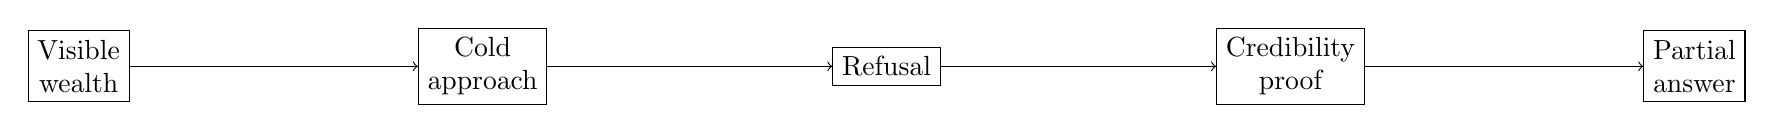
\begin{tikzpicture}[x=2.7cm,y=1.25cm]
\node[draw, align=center] (a) at (0,0) {Visible\\wealth};
\node[draw, align=center] (b) at (1.9,0) {Cold\\approach};
\node[draw, align=center] (c) at (3.8,0) {Refusal};
\node[draw, align=center] (d) at (5.7,0) {Credibility\\proof};
\node[draw, align=center] (e) at (7.6,0) {Partial\\answer};
\draw[->] (a) -- (b);
\draw[->] (b) -- (c);
\draw[->] (c) -- (d);
\draw[->] (d) -- (e);
\end{tikzpicture}
\caption{A transcript-derived access funnel. The lecture insists that even in a dense wealth field, doctrine appears only after repeated social friction.}
\end{figure}

\section{The Venture-Capital Interlude}

The first real breakthrough is short and compressed. A venture capitalist gives answers quickly, often while trying to leave. That matters. The advice arrives under time pressure, and so it should be read as a high-level screening rule, not as a complete theory of venture finance.

The first criterion is market opportunity. We can write the lecture's principle in a minimal editorial form:
\begin{equation}
P(\text{funding}) \uparrow
\qquad \text{as} \qquad
M_{\text{opp}} \uparrow,
\end{equation}
where \(M_{\text{opp}}\) is perceived market opportunity.

Then comes the second theme: AI. The VC says that anything to do with AI is currently a strong opportunity, and that if one is not using AI one is likely to be left behind. The lecture does not derive this claim mathematically, but it treats AI as an asymmetry-amplifier: a technology that changes the size of the reachable market.

The third theme is even more basic. Customer primacy overrides internal preference:
\begin{equation}
N_{\text{customers}} = 0
\qquad \Longrightarrow \qquad
\text{business} = 0.
\end{equation}
This is the most important sentence in the segment. It is also the segment's most portable one. The VC does not say ``employees first,'' ``culture first,'' or ``vision first.'' He says the customer comes first, because without purchase there is no business.

Finally, when the discussion turns from backing founders to raising capital from others, the rule becomes track record. The lecture's implied logic is simple: people give money to those who have already shown they can make money for other people.

\subsection{Question \& Answer}

\paragraph{Question.} What is the minimum credible signal that makes a founder or fund manager worth backing?

\paragraph{Answer.} In this lecture, the signal is not eloquence but compression into three tests: a large market opportunity, real contact with customer demand, and a track record that can be shown rather than promised. The host later reduces the segment even further: use AI, and put the customer first.

\section{How a Company With Tiny Revenue Sold for \(70\) Million Dollars}

Now the lecture slows down. This is the first place where the arithmetic is explicit enough to deserve real notes. A founder says he became rich young by building a point-of-sale device and selling the company for a little north of \(70\) million dollars. Then he gives numbers that make the deal appear impossible if we think only in ordinary startup metrics:
\begin{align}
V_{\text{exit}} &\gtrsim 70 \times 10^6 \ \text{dollars},\\
R &\approx 60 \times 10^3 \ \text{dollars},\\
C &\approx 17 \times 10^6 \ \text{dollars}.
\end{align}
Here \(R\) is reported revenue and \(C\) is the speaker's cumulative spend on the company. These are spoken figures, not audited statements, but they are the numerical center of the lecture.

The first thing to notice is how badly ordinary revenue explains the exit.

\paragraph{Worked example.} The revenue-to-exit multiple implied by the transcript is enormous:
\begin{align}
\frac{V_{\text{exit}}}{R}
&\approx
\frac{70 \times 10^6}{60 \times 10^3}
\approx 1.17 \times 10^3,\\
\frac{C}{R}
&\approx
\frac{17 \times 10^6}{60 \times 10^3}
\approx 2.83 \times 10^2.
\end{align}
So the lecture is not teaching a pleasant story about steadily compounding revenue. It is teaching a more difficult lesson: seller-side income can be tiny while buyer-side value is immense.

The founder explains this through ``fit and function.'' The buyer already had roughly \(11{,}000\) sales representatives and, according to the speaker, would otherwise have needed a process equivalent to adding another \(9{,}000\). The founder says that this avoided process was itself worth about \(70\) to \(80\) million dollars. The sale price was then not a reward for current revenue; it was a price placed on the buyer's saved friction.

\begin{definition}
We will call
\begin{equation}
V_{\text{buyer-side}}
\approx
V_{\text{fit}} + V_{\text{function}} + V_{\text{avoided friction}}
\end{equation}
the buyer-side value of the acquisition.
\end{definition}

\begin{remark}
This is a transcript-level reconstruction of the founder's logic, not a board equation from the lecture. But it is the cleanest way to express what the speaker means by ``fit and function'' and by the claim that price is only an issue if value is absent.
\end{remark}

\subsection{Question \& Answer}

\paragraph{Question.} How can a company with tiny revenue command a large exit?

\paragraph{Answer.} Because revenue is not the only variable in the bargain. In this story, the relevant quantity is not what the seller has already monetized, but what the buyer can avoid spending in delay, hiring, process cost, and organizational friction. A convenient compressed form is
\begin{equation}
V_{\text{exit}} \approx V_{\text{buyer-side}}.
\end{equation}
The lecture does not claim an exact valuation formula. It claims something more useful: a rational buyer can pay for a future capability that is worth far more to the buyer than the seller's trailing revenue would suggest.

\begin{figure}[h]
\centering
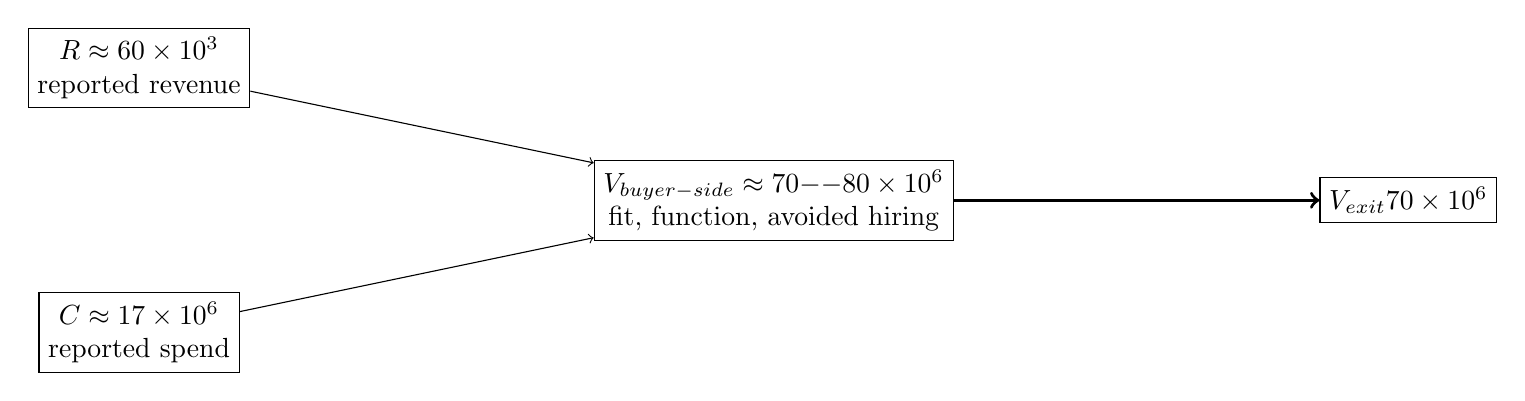
\begin{tikzpicture}[x=3.1cm,y=1.4cm]
\node[draw, align=center] (r) at (0,1.2) {$R \approx 60 \times 10^3$\\reported revenue};
\node[draw, align=center] (c) at (0,-1.2) {$C \approx 17 \times 10^6$\\reported spend};
\node[draw, align=center] (b) at (2.6,0) {$V_{\text{buyer-side}} \approx 70\text{--}80 \times 10^6$\\fit, function, avoided hiring};
\node[draw, align=center] (e) at (5.2,0) {$V_{\text{exit}} \gtrsim 70 \times 10^6$};
\draw[->] (r) -- (b);
\draw[->] (c) -- (b);
\draw[->, very thick] (b) -- (e);
\end{tikzpicture}
\caption{A transcript-derived reading of the point-of-sale exit. The lecture's surprise is that buyer-side savings dominate seller-side revenue.}
\end{figure}

The founder then widens the scale even further. He says he later built and sold five other companies, including one sale to Facebook, one to NetSuite/Oracle, and another exit around \(285\) million dollars. The point is not merely that he repeated the trick. It is that the lecture has now found a witness who can move from one surprising deal into a more general theory of value.

\section{Old Industry, Short Supply: Switchgear}

The same founder now shifts from software and exits into biography, industry selection, and manufacturing. He says he could not read until the ninth grade, had no parents, and effectively taught himself into entrepreneurship after a grandmother gave him a \(70{,}000\)-dollar check that he repaid in three months. This widening matters. The lecture is refusing to treat the arithmetic as detachable from the person who learned it.

When asked what industry matters now, the answer is not glamorous software. It is energy, infrastructure, and manufacturing, specifically switchgear. The speaker's thesis is that an old, low-technology space can become extraordinarily lucrative when demand outruns supply for structural reasons.

The central numerical claim concerns capacity. A study attributed to Amazon is summarized this way: even if Amazon absorbed all United States switchgear manufacturing capacity over the next ten years, it would still satisfy only about \(25\%\) of its need. In symbols,
\begin{equation}
\frac{K_{\text{available}}}{D_{\text{Amazon need}}} \approx 0.25.
\end{equation}
Rearranging gives the implied gap:
\begin{equation}
D_{\text{Amazon need}} \approx 4 K_{\text{available}}.
\end{equation}
That is the heart of the segment. The field is attractive because shortage is not incidental. It is built into the present scale of digital infrastructure demand.

The speaker then gives the economics of his own position in the space:
\begin{align}
K_{\text{rev}} &\approx 1.2 \times 10^9 \ \text{dollars},\\
\rho_g &\approx 0.5.
\end{align}
Here \(K_{\text{rev}}\) is stated revenue capacity and \(\rho_g\) is gross margin. The implied gross-profit capacity is therefore
\begin{equation}
\Pi_g \approx \rho_g K_{\text{rev}}
\approx 0.5 \times 1.2 \times 10^9
\approx 0.6 \times 10^9 \ \text{dollars}.
\end{equation}
This is why the speaker says he is getting ``software money out of manufacturing.'' The phrase is not metaphorical. It refers to the combination of shortage, selective clientele, and unusually large gross margins.

The ticket sizes reinforce the scale:
\begin{align}
P_{\text{building switchgear}} &\approx 15 \times 10^6 \ \text{dollars},\\
P_{\text{small data center}} &\approx 15\text{--}20 \times 10^6 \ \text{dollars},\\
P_{\text{large data center}} &\approx 1 \times 10^9 \ \text{dollars}.
\end{align}
The lecture's argument is now clear. A dull object can become a highly intelligent business if it sits at a choke point in a growing system.

\subsection{Question \& Answer}

\paragraph{Question.} Why can an old industrial product generate software-like money?

\paragraph{Answer.} Because ``old'' does not mean ``commoditized'' when demand is exploding and capacity is scarce. The lecture's switchgear example combines replacement demand, new data-center demand, high ticket size, and the inability of incumbent supply to keep up. In that environment, margins can remain unexpectedly large.

The founder also mentions a current company growing along the ladder
\begin{equation}
5 \times 10^6 \to 50 \times 10^6 \to 300 \times 10^6
\end{equation}
in successive stages. The point of this growth ladder is not audited forecasting. It is a scale transition: once the field is right, growth can move by order-of-magnitude jumps rather than by linear increments.

The lecture then widens once more, away from business arithmetic and into faith. The same speaker says the Bible changed his life and offers an explicit Christian apologetic argument about design and creator. Whether one agrees is secondary for present purposes. Structurally, the lecture is showing us that the same person who reasons in margins and capacity also reasons in vocation, biography, and metaphysics.

\paragraph{Interruption.} At this point the lecture breaks into a long promotional appeal for a mentorship community. In the notes we should neither ignore nor expand this too much. Its structural meaning is simple: hard-won access is being turned into a sellable promise of proximity.

\section{Two Other Routes: Apple and Satellites}

After the interruption the lecture returns to the field and deliberately broadens its taxonomy of wealth. We are no longer in a single-founder world.

\paragraph{The Apple route.} The Ferrari owner in the resumed segment did not make his money by founding the firm in question. He worked at Apple, rose to engineering director, stayed for almost two decades, and says his wealth vehicle was Apple stock. The lecture's cleanest editorial compression is
\begin{equation}
W_{\text{employee}} \approx Y_{\text{salary}} + G_{\text{stock}},
\end{equation}
with the important warning that the second term is doing most of the asymmetry.

The tenure number is explicit:
\begin{equation}
t_{\text{Apple}} \approx 20 \ \text{years}.
\end{equation}
This is a very different wealth mechanism from the exit story. One gets rich here not by selling a firm but by attaching oneself, early and for a long time, to an extraordinary company. The speaker's advice is also notably different from the VC's enthusiasm about AI. He says that when everyone is on the AI bandwagon, it may no longer be the best place to look, and he gives a classic Apple lesson: set a high bar.

\paragraph{The satellite route.} The next speaker says he made it later in life, perhaps around fifty, by building a satellite company. The origin story is striking. After \(9/11\) he found a company that was broken and believed the world would need more information about people and places. He says he did not initially realize it would make a great deal of money.

The scale markers are rough but important:
\begin{align}
V_{\text{government contract}} &\in \text{``billions of dollars''},\\
T_{\text{work}} &\in \{6,7\} \ \text{days per week}.
\end{align}
The lecture couples these with sacrifice: years of six- or seven-day workweeks, missed family events, and the claim that the effort made the country safer, protected the environment, created jobs, and enriched investors.

\subsection{Question \& Answer}

\paragraph{Question.} What makes a broken business worth fixing rather than abandoning?

\paragraph{Answer.} In the lecture's answer, a broken business becomes worth fixing when it is misaligned with what the customer actually needs. The satellite founder gives the principle explicitly:
\begin{equation}
\text{commercial fit} \uparrow
\qquad \text{as} \qquad
\|\text{offer} - \text{customer need}\| \downarrow.
\end{equation}
He says businesses are broken because they sell what they have, not what the customer needs. In his case the unmet need was information: digital maps, geographic knowledge, and situational visibility at a time when people did not yet take such tools for granted.

This is also why the lecture does not reduce the story to luck. Luck matters, but the commercial mechanism is still legible. The firm won because it aligned supply with a need that the customer had not yet fully articulated. The same speaker then adds a forward-looking industry claim: cyber will become more important because AI makes deception easier.

\section{Happiness as a Business Variable}

The lecture closes by moving away from founders, funds, and infrastructure and toward service. A plastic surgeon says he was a farm boy from Illinois, had a misspent youth, worked hard, and made his patients happy. In the lecture's final movement, Silicon Valley wealth is shown to include medicine and direct service as well as software and capital.

The most concrete number in this section is a ticket size:
\begin{equation}
P_{\text{surgery}} \approx 20{,}000 \ \text{dollars}.
\end{equation}
Patients, he says, arrive with cash for surgery, and many are ordinary hard-working business owners rather than glamorous elites. The important point is not simply that the procedure is expensive. It is that high willingness to pay can coexist with perceived benefit.

\subsection{Question \& Answer}

\paragraph{Question.} Can making people happier be a real business model rather than a sentimental slogan?

\paragraph{Answer.} In the lecture's final answer, yes. The surgeon does not deny that money is made. He says instead that happiness may matter more than the money. The commercial claim is softer than the switchgear claim, but it is still recognizable: when one enjoys the work, gets good at it, and delivers visibly better outcomes, people become willing to pay substantial amounts and to reward the practice. A cautious editorial version is
\begin{equation}
\text{service strength} \uparrow
\qquad \text{as} \qquad
\text{client happiness} \uparrow.
\end{equation}

The speaker also emphasizes the role of technology. Better tools improve healing, improve results, and therefore improve patient satisfaction. This does not become a formal derivation in the lecture, but it nicely mirrors earlier sections: whether in Apple, satellites, switchgear, or surgery, technology matters when it amplifies a real need rather than merely decorating a story.

\section{Summary}

The lecture begins with spectacle but does not stay there. It moves from Ferrari-scale outcomes to a much more interesting claim: wealth comes through identifiable mechanisms, and those mechanisms differ sharply. Venture capital screens for market opportunity, customer purchase, and track record. A founder can sell a company for tens of millions on almost no revenue if the buyer-side savings are large enough. An old industrial product can become a high-margin gold mine when demand outruns capacity. An employee can become rich through long-duration exposure to stock appreciation. A founder can repair a broken company by selling what customers need rather than what the company happens to have. A surgeon can build a lucrative practice by making people happier.

The central discipline of the lecture is therefore not hype but discrimination. We should not ask only where money is visible. We should ask what structure makes the money possible: market size, bottleneck, buyer-side value, stock exposure, institutional demand, or service quality. Once we begin asking that question, Silicon Valley ceases to be a mythic landscape and becomes what the lecture is really trying to show us: a dense field of commercial mechanisms.